\documentclass{article}

\usepackage[english]{babel}
\usepackage[utf8]{inputenc}
\usepackage[T1]{fontenc}
\usepackage{amsmath, amsfonts, amssymb, amsthm}
\usepackage{tikz}
\usepackage{csquotes}

\usepackage[backend=biber,citetracker=true]{biblatex}
\addbibresource{bibli.bib}
\usepackage{color}
\usepackage{subcaption}
\usepackage{graphicx}
\usepackage{./tex/sty/scribe}
\usepackage{float}

\newcommand*{\AIC}{\mathrm{AIC}}
\newcommand*{\BIC}{\mathrm{BIC}}

%\usepackage{epsfig}
%\usepackage{ulem, stmaryrd, dsfont}


\author{Fanchon Herman}


\begin{document}
\begin{titlepage} 
	\newcommand{\HRule}{\rule{\linewidth}{0.5mm}}
	
	\center
	
	\textsc{\LARGE University of Montpellier}\\[1.5cm]
	
	\textsc{\Large Master 2 Biostatistique }\\[0.5cm] 
	
	\textsc{\large HMMA$307$ Project}\\[0.5cm] 

	\HRule\\[0.4cm]
	
	{\huge\bfseries Linear Mixed Models}\\[0.4cm] 
	
	\HRule\\[1.5cm]
	
	\begin{minipage}{0.4\textwidth}
		\begin{flushleft}
			\large
			\textit{Student: }\\
			Fanchon Herman
		\end{flushleft}
	\end{minipage}
	~
	\begin{minipage}{0.4\textwidth}
		\begin{flushright}
			\large
			\textit{Teacher: }\\
			Joseph Salmon\\
		\end{flushright}
	\end{minipage}
		\vfill 
	
	{\large 2020-2021} 

		\vfill\vfill
		
\centering

\includegraphics[width=0.2\textwidth]{./images/Logo}


	
	 
	%----------------------------------------------------------------------------------------
	
	\vfill 
\end{titlepage}

\tableofcontents
\newpage
%%%%%%%%%%%%%%%%%%%%%%%%%%%%%%%%%%%%%%%%%%%%%%%%%%%%%%%%%%%%%%%%%%%%%%%%%%%%%%%
%%%%%%%%%%%%%%%%%%%%%%%%%%%%%%%%%%%%%%%%%%%%%%%%%%%%%%%%%%%%%%%%%%%%%%%%%%%%%%%
\section*{Introduction}

Linear mixed models are an extension of simple linear models to allow for fixed effects and random effects. A fixed effect is a parameter that remains constant and random effects are parameters that are random variables.These types of models are widely used when the data is not independent.

In this project, we use the dataset from Grodner and Gibson, Expt $1$.
This dataset deals with subject and object relative clause data from English.
Grodner and Gibson analyzed the reading times at the relative clause verb in a self-paced reading study. In this dataset, we have $672$ observations and $42$ subjects.

Throughout this project, we are interested in three main types of linear mixed models. For each models, we will explain the statistical model and the model outputs on $\texttt{Python}$. In addition, we take care to validate the model and select the most judicious model using various criteria.
%%%%%%%%%%%%%%%%%%%%%%%%%%%%%%%%%%%%%%%%%%%%%%%%%%%%%%%%%%%%%%%%%%%%%%%%%%%%%%%
%%%%%%%%%%%%%%%%%%%%%%%%%%%%%%%%%%%%%%%%%%%%%%%%%%%%%%%%%%%%%%%%%%%%%%%%%%%%%%%


%%%%%%%%%%%%%%%%%%%%%%%%%%%%%%%%%%%%%%%%%%%%%%%%%%%%%%%%%%%%%%%%%%%%%%%%%%%%%%%
%%%%%%%%%%%%%%%%%%%%%%%%%%%%%%%%%%%%%%%%%%%%%%%%%%%%%%%%%%%%%%%%%%%%%%%%%%%%%%%
\section{Model type 1 - Varying intercepts}
We first start to analyze a mixed linear model by varying the intercept.
We modeling individual means with random intercepts.
So, the previous statement adjusts the grand mean estimates of the intercept by a term for each subject. Only the mean and standard deviation of the intercept distribution are estimated instead of $42$ intercepts for each subject.
This saves degrees of freedom because less parameter estimation is required.
We  model these individual differences by assuming different random intercepts for each subject. So, each subject is assigned a different intercept value.

\subsection{Mathematical equation of the model}
The mathematical equation of the model is:
\[y_{ij}= \beta_0 + u_{0i} + \beta_1 \times so_{ij} + \varepsilon_{ij},\]
In this model, $i$ indexes subjects and $j$ indexes items. So, $i \in [1,42]$ and $j \in [1,16].$
Besides, the intercept $\beta_0$ and $so_{ij}$  represent two fixed effects and $u_{0i}$ represent a random effect. The model has a different intercept $\beta_0 + u_{i0}$ for each subject $i$. In addition, $\beta_1$ correspond to the slope parameter.

In the model above, we have two sources of variance which are :
\begin{itemize}
    \item $u_{0i} \sim \mathcal{N}(0,\sigma_{u0}) \text{ , } \sigma_{u0}>0$, iid on $i$,
    \item $\varepsilon \sim \mathcal{N}(0, \sigma) \text{ , } \sigma >0$, iid on $i$ and $j$,
    \item $\forall i \text{,} j \text{ , } u_{i0} \perp \!\!\! \perp \varepsilon_{ij}$.
\end{itemize}

In addition, these two standard deviations determine the standard error of the $\beta_1$ slope parameter.

From the model above, we can calculate its expectation and its variance: 
$$\E(y_{ij})=\beta_0 + \beta_1 \E(so_{ij})$$
$$\Var(y_{ij})=\sigma_{u0} + \beta_1^2 Var(so_{ij}) + \sigma$$

\subsection{Model explanations}
The output of the model is:
\begin{center}
    \begin{tabular}{|c|c|c|c|c|c|}
    \hline
         & Coef & Std.Err & z & P>|z| &[0.025 0.975]  \\
         \hline \hline
        Intercept & 5.883 & 0.051 & 115.502 & 0.000 & 5.783 5.983\\
         so & 0.062 & 0.015 & 4.205 & 0.000 & 0.033 0.091 \\
         Group var &  0.100 & 0.065 &  & &  \\
         \hline
    \end{tabular}
    \captionof{table}{Numerical outputs of the mixed linear model carried out on \texttt{Python}.} 
\end{center}


By the results of the mixed linear model, we have:
$\hat{\sigma}_{u0}=0.316$ and $\hat{\sigma}=0.382$.

The theoretical formulas of the estimators are:
\begin{itemize}
    \item $\hat{\sigma}=\dfrac{1}{n-J} \sum_{j=1}^{J} \sum_{i=1}^{n_j} (y_{ij}-\Bar{y}_{:j})^2$,
    \item $\hat{\sigma}_{u0}=\dfrac{\dfrac{1}{J-1} \sum_{j=1}^J n_j(\Bar{y}_{:j}-y_n)^2 - \hat{\sigma}}{n^2 - \sum_{j=1}^J n_j^2}$,
\end{itemize}
where $n_j$ corresponds to the number of repetitions of the phenomenon, $n=\sum_{j=1}^J n_j$ and $\Bar{y}_{:j}=\dfrac{1}{n_j}\sum_{i=1}^{n_j} y_{ij}$.

In addition, we can see that the intercept (subject) explain around $40\%$ of the variations. Indeed, we have: $\dfrac{\hat{\sigma}_{u0}^2}{\hat{\sigma}_{u0}^2+\hat{\sigma}^2}=\dfrac{0.0999}{0.0999+0.146} \simeq 0.4$.
So, after the variance explained by fixed effects, the differences between the subjects explain about $40\%$ of the remaining variance.

We can also see that the confidence interval of the variable so is $[0.033, 0.091]$. The latter does not include the value $0$, so we can say that is significantly différent from $0$.

Now, let's visualize the adjustments to the grand mean for each subject.

\begin{figure}[H]
    \centering
    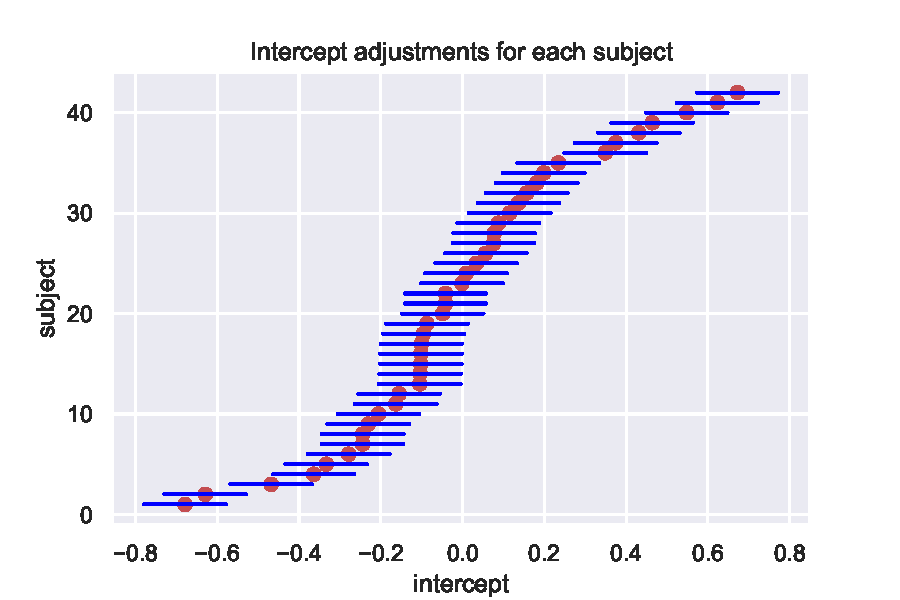
\includegraphics[scale=.65]{./images/model1_inter.pdf}
    \caption{Representation of the intercept adjustements by subject.}
    \label{fig:model1}
\end{figure}

In the Figure \ref{fig:model1}, we can note that our model produces a different intercept for each subjects in addition to a parameter estimate for features logrt (log-transformed reading time) and so (the contrast coding) which is constant between subjects. In addition, the error bars represent $95\%$ confidence intervals. We can see that there is a large variability in the average reading times between subjects.

\subsection{Model validation}
Now, see how can we validate the model. In order to check the homogeneity, we plot the predicted values versus the residuals. In addition, we also check the normality of the residuals.
\begin{figure}[H]
\centering
\begin{subfigure}{.5\textwidth}
  \centering
  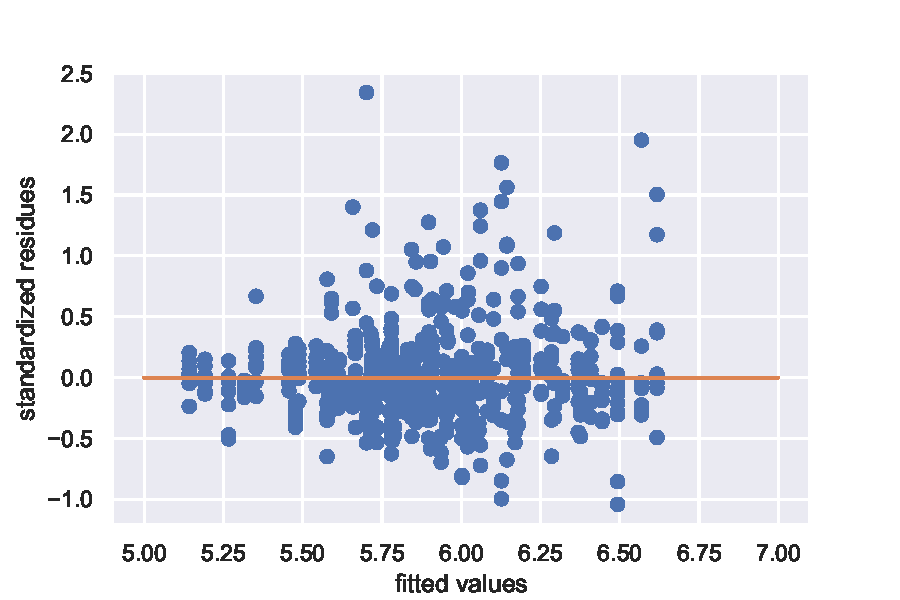
\includegraphics[width=1\linewidth]{./images/homo_mod1.pdf}
  \caption{Representation of the predicted by residual values.}
  \label{fig:homo_mod1}
\end{subfigure}%
\begin{subfigure}{.5\textwidth}
  \centering
  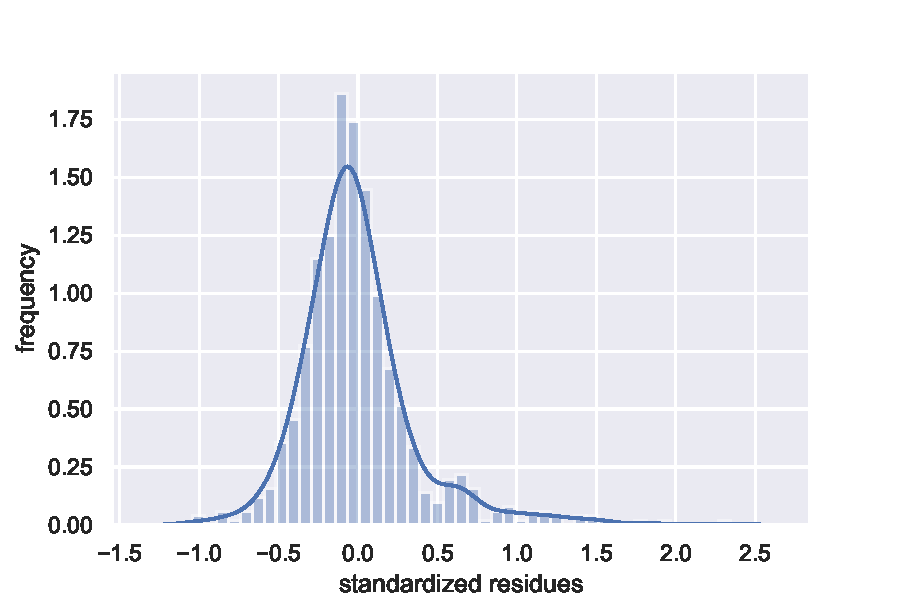
\includegraphics[width=1\linewidth, clip,trim={0cm 0cm 0cm 0.6cm} ]{./images/resid_norm.pdf}
  \caption{Representation of the normality of the residuals.}
  \label{fig:resid}
\end{subfigure}
\caption{Model validation.}
\label{fig:valid_1}
\end{figure}

In the Figure \ref{fig:valid_1}, we can note that the magnitude of the residuals suggests that the model seems to model our data well. In addition, we can see that the normality of the residuals is verified.

\subsection{Model selection}
In order to evaluate the models, we can use the AIC criterion.
So, we calculate the AIC of the model above to compare it with those of the other models defined in the other parts below. The AIC criterion is defined by:
\[ \AIC = 2k - 2\ln({\hat{L}}),\]
with  $k$ is the number of estimated parameters in the model and $\hat{L}$ is the maximum likelihood of the model.


For practical reasons, we use the AIC formula defined using the deviance:
$$\AIC=\text{deviance} + 2 \times (p+1)=2 \times \log(\text{likelihood}) + 2 \times (p+1).$$
In the formula, $1$ corresponds to the estimated residual variance and $p$ is all the other parameters.


Using the above formula and for our associated model, we find an AIC of approximately $735.6817$ (with a total of $4=3+1$ parameters).

We can also use the BIC criterion for model selection. The BIC criterion is defined by:
\[ \BIC= (-2) \times \text{loglikehood} + (p+1) \times \ln(n).\]
where $1$ corresponds to the estimated residual variance, $p$ is all the other parameters estimate and $n$ is the number of observations.
For our model, the BIC is approximately equal to $753.7227$.

%%%%%%%%%%%%%%%%%%%%%%%%%%%%%%%%%%%%%%%%%%%%%%%%%%%%%%%%%%%%%%%%%%%%%%%%%%%%%%%
%%%%%%%%%%%%%%%%%%%%%%%%%%%%%%%%%%%%%%%%%%%%%%%%%%%%%%%%%%%%%%%%%%%%%%%%%%%%%%%

%%%%%%%%%%%%%%%%%%%%%%%%%%%%%%%%%%%%%%%%%%%%%%%%%%%%%%%%%%%%%%%%%%%%%%%%%%%%%%%
%%%%%%%%%%%%%%%%%%%%%%%%%%%%%%%%%%%%%%%%%%%%%%%%%%%%%%%%%%%%%%%%%%%%%%%%%%%%%%%
\section{Model type 2 - Varying intercepts and slopes, without a correlation}

The first model suppose different intercepts by subjects. However, the slope remained the same for each subject. So, we will now study a second type of model by varying the intercepts and slopes, without correlation. 
As with the intercepts, only the mean and standard deviation of the slopes are estimated instead of $42$ separate slopes.

\subsection{Mathematical equation of the model}
The mathematical equation of the model is:
\[y_{ij}= \beta_0 + u_{0i} + (\beta_1 + u_{1i}) \times so_{ij} + \varepsilon_{ij},\]
In this model, $i$ indexes subjects and $j$ indexes items. So, $i \in [1,42]$ and $j \in [1,16]$.

In the model above, we have three sources of variance which are :
\begin{itemize}
    \item $u_0 \sim \mathcal{N}(0,\sigma_{u0})$, $\sigma_{u0}>0$,
    \item $u_1 \sim \mathcal{N}(0,\sigma_{u1})$, $\sigma_{u1}>0$,
    \item $\varepsilon \sim \mathcal{N}(0, \sigma)$, $\sigma>0$.
\end{itemize}

\subsection{Model explanations}
The output of the model is:
\begin{center}
    \begin{tabular}{|c|c|c|c|c|c|}
    \hline
         & Coef & Std.Err & z & P>|z| & [0.025 0.975]  \\
         \hline \hline
        Intercept & 5.883 & 0.051 & 115.496 & 0.000 & 5.783 5.983\\
         so & 0.062 & 0.022 & 2.810 & 0.005 & 0.019 0.105 \\
         Group var &  0.101 & 0.068 &  & & \\
         Group x so Cov & 0.020 & 0.022 & & &\\
         so Var & 0.012 & 0.013 & & &\\
         \hline
    \end{tabular}
    \captionof{table}{Numerical outputs of the mixed linear model carried out on \texttt{Python}.} 
\end{center}

First, by the results of the mixed linear model, we have:
$\hat{\sigma}_{u0}=0.317$, $\hat{\sigma}_{u1}=0.110$ and $\hat{\sigma}=\sqrt{0.1336}=0.366$.

In addition, we can see that the intercept(subject) and the adjusted slope by subjects explain around $50\%$ of the variations. Indeed, we have: $\dfrac{\hat{\sigma}_{u0}^2}{\hat{\sigma}_{u0}^2+\hat{\sigma}^2} + \dfrac{\hat{\sigma}_{u1}^2}{\hat{\sigma}_{u1}^2+\hat{\sigma}^2} =\dfrac{0.1005}{0.1005+0.1336} + \dfrac{0.0121}{0.0121+0.1336} \simeq 0.5$.
So, after the variance explained by fixed effects, the differences between the subjects and the adjusted slope by subjects explain almost $50\%$ of the remaining variance.

In order to determine if the slope is significantly different from $0$ or not, we will study its confidence interval.
Indeed, if its confidence interval includes the value $0$, we can say that the slope is not significantly different from $0$.
The confidence interval of the slope is $[0.019, 0.105]$. So, as the latter does not include $0$, we can affirm at the $5\%$ threshold that the slope is significantly different from $0$.

Let's visualize the adjustments to the intercept and slope for each subject.

\begin{figure}[H]
    \centering
    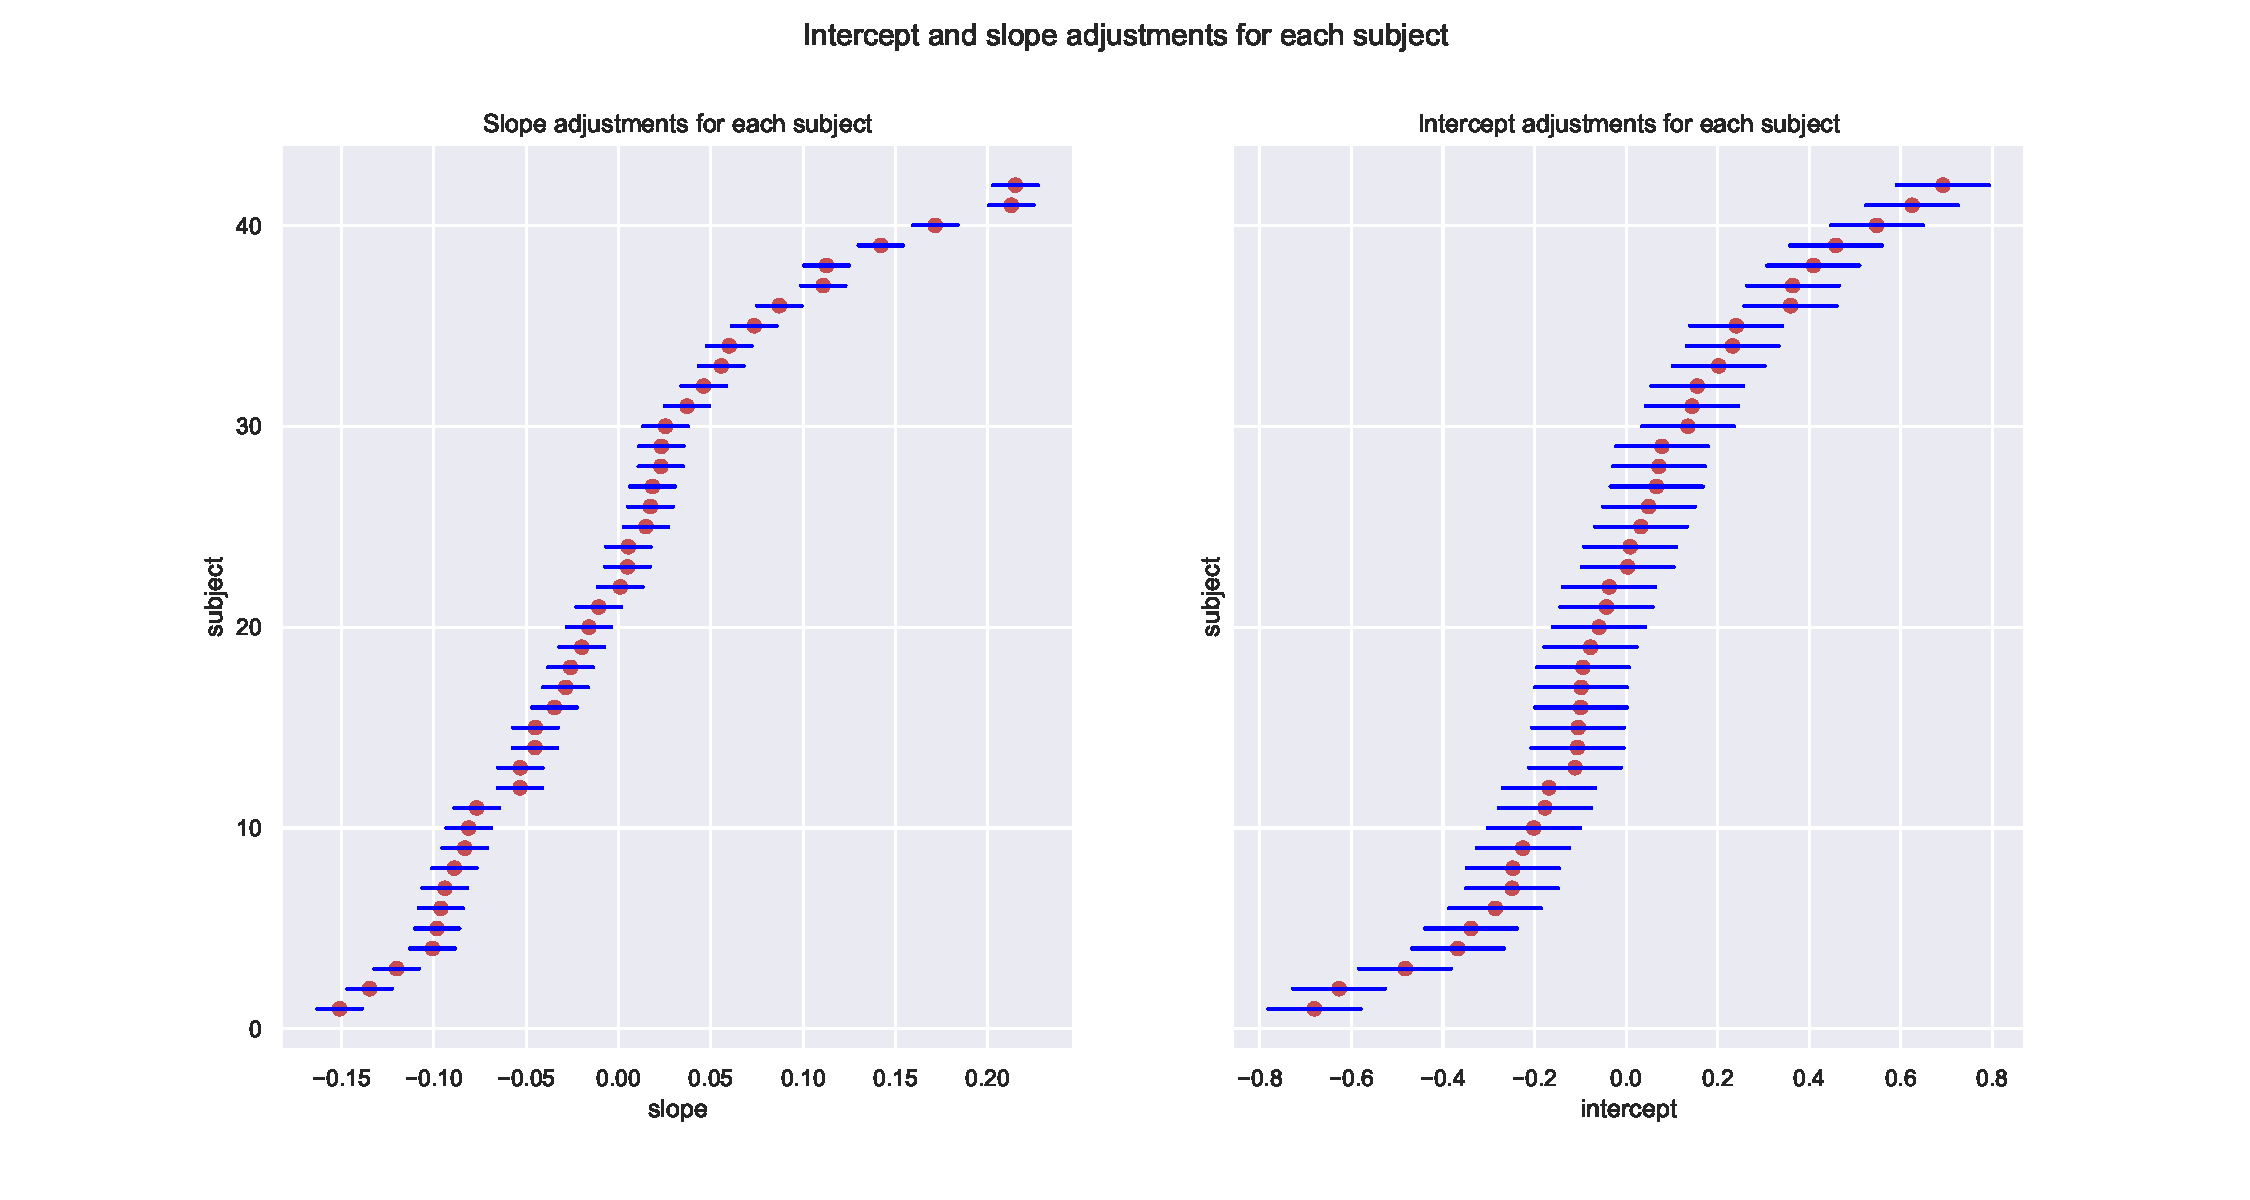
\includegraphics[scale=.42]{./images/model2_inter.pdf}
    \caption{Representation of the intercept and slope adjustements by subject.}
    \label{fig:model2}
\end{figure}

In the Figure \ref{fig:model2}, we can note a little variation in slope between subjects. However, there is a large variability in the average reading times between subjects. Like the previous model, we can note that our model produces a different intercept and slope for each subjects in addition to a parameter estimate for features logrt (log-transformed reading time) and so (the contrast coding) which is constant between subjects. The error bars in the figure represent $95\%$ confidence intervals.

\subsection{Model validation}
As before, we try to validate our model.
We are going to plot the predicted values versus the residuals to check the homogeneity. Moreover, we also check the normality of the residues.

\begin{figure}[H]
\centering
\begin{subfigure}{.5\textwidth}
  \centering
  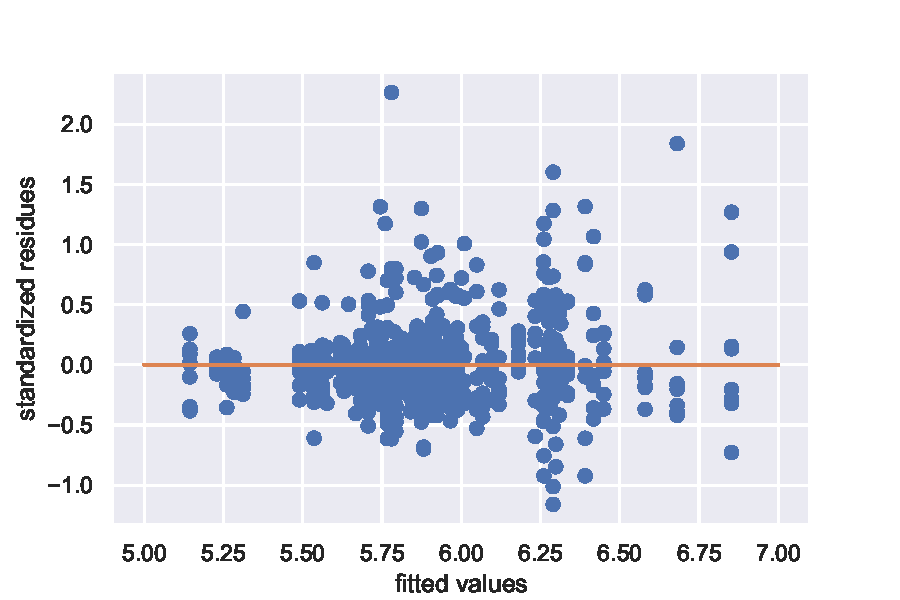
\includegraphics[width=1\linewidth]{./images/homo_mod2.pdf}
  \caption{Representation of the predicted by residual values.}
  \label{fig:homo_mod2}
\end{subfigure}%
\begin{subfigure}{.5\textwidth}
  \centering
  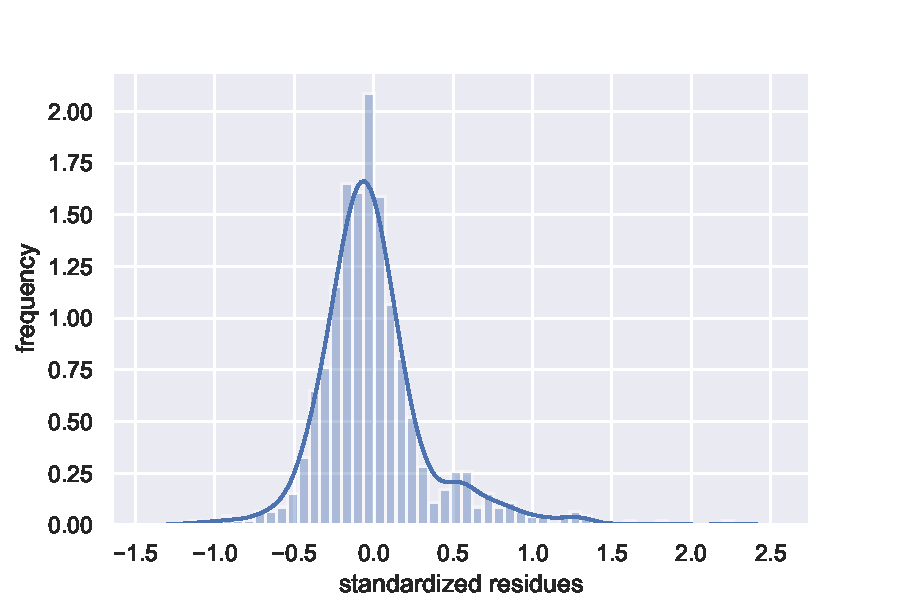
\includegraphics[width=1\linewidth, clip,trim={0cm 0cm 0cm 0.6cm} ]{./images/resid_norm_m2.pdf}
  \caption{Representation of the normality of the residuals.}
  \label{fig:resid_}
\end{subfigure}
\caption{Model validation.}
\label{fig:valid_2}
\end{figure}

In the Figure \ref{fig:valid_2}, we can note that the residuals seem to be not too far from the orange line. Meaning that the model fits our data well.
Moreover, the normality of the residuals is also check.

\subsection{Model selection}
After studying two different models, we can compare these two models by comparing their AIC values.
Using the AIC formula defined from the deviance, we obtain an AIC of approximately $711.1463$. In addition, the value of the BIC criterion is approximately equal to $738.2079$.
Since the previous model has a greater AIC and BIC values than this, we can say that this model is the "best" model for our data. Thus, this model has a greater predictive power than the previous model.

%%%%%%%%%%%%%%%%%%%%%%%%%%%%%%%%%%%%%%%%%%%%%%%%%%%%%%%%%%%%%%%%%%%%%%%%%%%%%%%
%%%%%%%%%%%%%%%%%%%%%%%%%%%%%%%%%%%%%%%%%%%%%%%%%%%%%%%%%%%%%%%%%%%%%%%%%%%%%%%


%%%%%%%%%%%%%%%%%%%%%%%%%%%%%%%%%%%%%%%%%%%%%%%%%%%%%%%%%%%%%%%%%%%%%%%%%%%%%%%
%%%%%%%%%%%%%%%%%%%%%%%%%%%%%%%%%%%%%%%%%%%%%%%%%%%%%%%%%%%%%%%%%%%%%%%%%%%%%%%
\section{Model type 3 - Varying intercepts and varying slopes, with correlation}
%%%%%%%%%%%%%%%%%%%%%%%%%%%%%%%%%%%%%%%%%%%%%%%%%%%%%%%%%%%%%%%%%%%%%%%%%%%%%%%
%%%%%%%%%%%%%%%%%%%%%%%%%%%%%%%%%%%%%%%%%%%%%%%%%%%%%%%%%%%%%%%%%%%%%%%%%%%%%%%

\subsection{Mathematical equation od the model}
The mathematical equation of the model is:
\[y_{ij}= \alpha + u_{0i} + w_{0j}+(\beta + u_{1i} + w_{1j}) \times so_{ij} + \varepsilon_{ij},\]
with 
\begin{itemize}
    \item $\varepsilon_{ij} \sim \mathcal{N}(0, \sigma)$, $\sigma>0$,
    \item
    $\begin{pmatrix}
    u_0\\
    u_1\\
    \end{pmatrix}\sim \mathcal{N}\left(\begin{pmatrix}
    0\\
    0\\
    \end{pmatrix},\Sigma_u\right)$,
    \item 
    $\begin{pmatrix}
    w_0\\
    w_1\\
    \end{pmatrix}\sim \mathcal{N}\left(\begin{pmatrix}
    0\\
    0\\
    \end{pmatrix},\Sigma_w\right)$.
\end{itemize}
where $\Sigma_u=\begin{pmatrix}
\sigma_{u0}^2  & \rho_u\sigma_{u0}\sigma_{u1}\\
\rho_u\sigma_{u0}\sigma_{u1} & \sigma_{u1}^2\\
\end{pmatrix} \text{ and } \begin{pmatrix}
\sigma_{w0}^2  & \rho_u\sigma_{w0}\sigma_{w1}\\
\rho_u\sigma_{w0}\sigma_{w1} & \sigma_{w1}^2\\
\end{pmatrix} $

In this model, $i$ indexes subjects and $j$ indexes items. So, $i \in [1,42]$ and $j \in [1,16]$. 
In this model, we add item-level effects and also include correlation parameters.

\subsection{Model explanations}
The output of the model is:
\begin{center}
    \begin{tabular}{|c|c|c|c|c|c|}
    \hline
         & Coef & Std.Err & z & P>|z| & [0.025 0.975]  \\
         \hline \hline
        Intercept & 5.883 & 0.051 & 115.497 & 0.000 & 5.783 5.983\\
         so & 0.062 & 0.022 & 2.810 & 0.005 & 0.019 0.105 \\
         subject var &  0.101 &  &  & & \\
         subject x so Cov & 0.020 &  & & &\\
         so Var & 0.012 &  & & &\\
         item Var & 0.076 & & & &\\
         \hline
    \end{tabular}
    \captionof{table}{Numerical outputs of the mixed linear model carried out on \texttt{Python}.} 
\end{center}

Let's visualize the adjustments to the intercept and slope for each subject.

\begin{figure}[H]
    \centering
    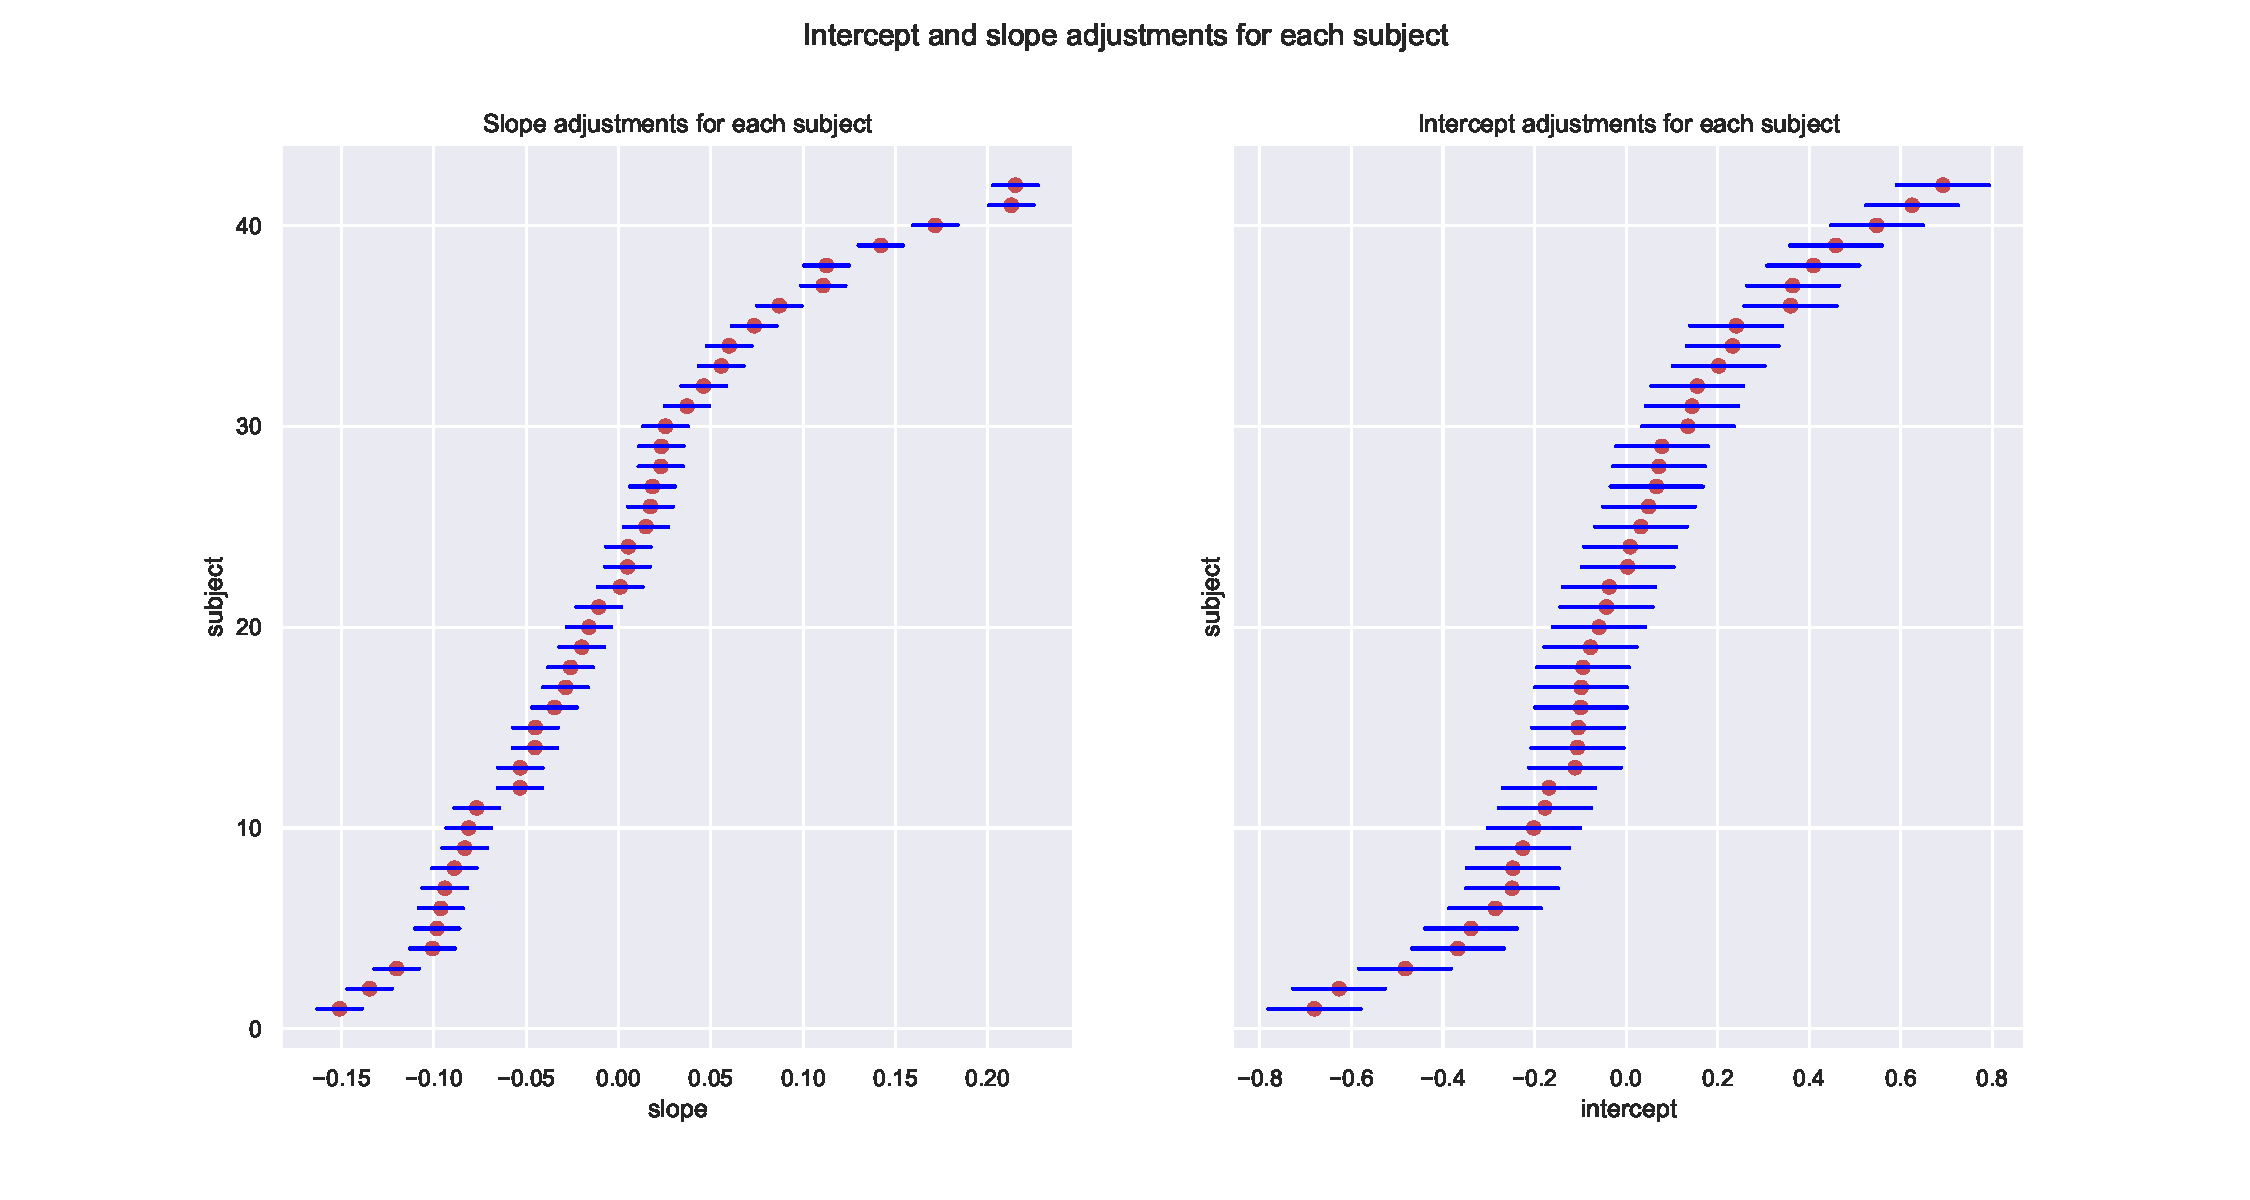
\includegraphics[scale=.42]{./images/model3_inter.pdf}
    \caption{Representation of the intercept and slope adjustements by subject.}
    \label{fig:model3}
\end{figure}

In the Figure \ref{fig:model3}, we can note a little variation in slope between subjects and  a large variability in the average reading times between subjects. Like the previous model, we can note that our model produces a different intercept and slope for each subjects. The error bars in the figure represent $95\%$ confidence intervals.


In order to visualize the correlation between intercept and slopes by subjects, we plot the slope adjustments against the intercept adjustments.
\begin{figure}[H]
    \centering
    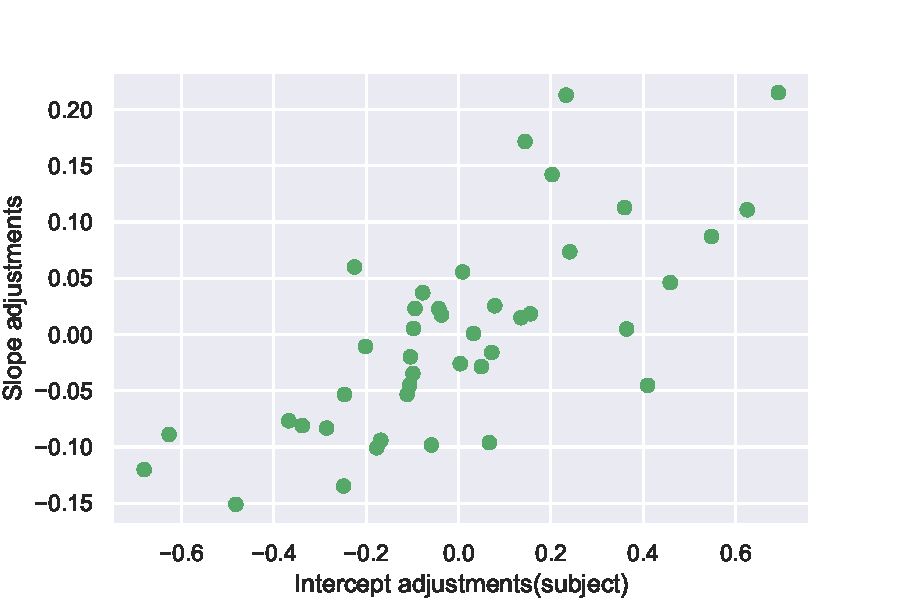
\includegraphics[scale=.65]{./images/adj_so_inter.pdf}
    \caption{Representation of the slope adjustments against the intercept adjustements.}
    \label{fig:adj_slope}
\end{figure}

On the Figure \ref{fig:adj_slope}, we can recognize the data could fit a linear model. Indeed, considering that there is some noise on the data, when the intercept gets higher, the slope adjustement also increase linearly. 

\subsection{Model validation}
Now, we are going to validate this model. To do this, we plot the predicted values versus the residuals to check the homogeneity and we also check the normality of the residues.

\begin{figure}[H]
\centering
\begin{subfigure}{.5\textwidth}
  \centering
  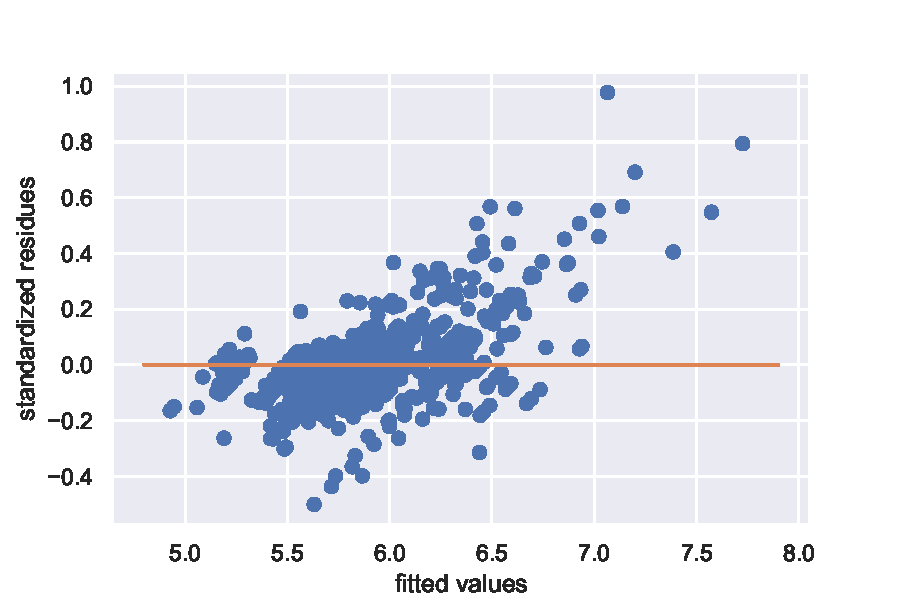
\includegraphics[width=1\linewidth]{./images/homo_mod3.pdf}
  \caption{Representation of the predicted by residual values.}
  \label{fig:homo_mod3}
\end{subfigure}%
\begin{subfigure}{.5\textwidth}
  \centering
  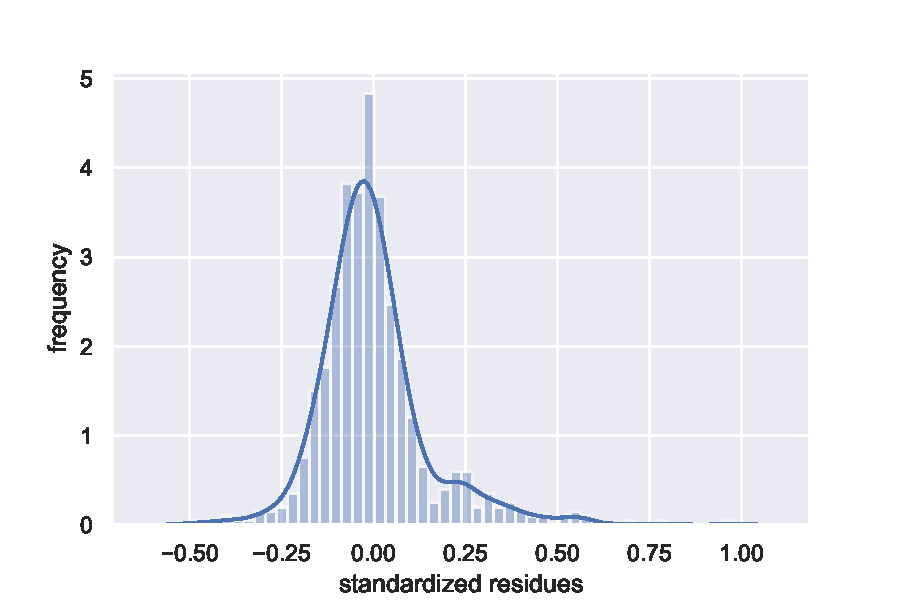
\includegraphics[width=1\linewidth, clip,trim={0cm 0cm 0cm 0.6cm} ]{./images/resid_norm_m3.pdf}
  \caption{Representation of the normality of the residuals.}
  \label{fig:resid3}
\end{subfigure}
\caption{Model validation.}
\label{fig:valid_3}
\end{figure}

In the Figure \ref{fig:valid_3}, we can see that the residues are particularly clustered around the orange line. So our model fits the data well. In addition, the normality of the residuals is also verified..

\subsection{Model selection}
We studied a total of three different models. In order to know which model is the most judicious, we compare the values of the criterion AIC and BIC.
For this model, we obtain an AIC approximately equal to $717.1464$ and a BIC approximately equal to $757.7386$. By comparing the AIC and BIC values of the other two models above, note that the model having a minimal AIC and also a minimal BIC is the second model. Recall that the second model is the model where varying intercepts and slopes, without correlation. Therefore, this second model has a greater predictive power than the other models.


%%%%%%%%%%%%%%%%%%%%%%%%%%%%%%%%%%%%%%%%%%%%%%%%%%%%%%%%%%%%%%%%%%%%%%%%%%%%%%%
%%%%%%%%%%%%%%%%%%%%%%%%%%%%%%%%%%%%%%%%%%%%%%%%%%%%%%%%%%%%%%%%%%%%%%%%%%%%%%%
\section*{Conclusion}
To sum up all of it, we have studied three different types of models which are:
varying intercepts, varying intercepts and slopes, without correlation and Varying intercepts and slopes, with correlation. 
For each of these, we have seen their statistical models but also how to validate the models. Moreover, we used two different criteria which are AIC and BIC in order to select the least worse model for our data. Thus, in view of the values of the AIC and BIC for the three models, we can say that the model with the least worse model is the second model  corresponding to varying intercepts and slopes, without correlation.

%%%%%%%%%%%%%%%%%%%%%%%%%%%%%%%%%%%%%%%%%%%%%%%%%%%%%%%%%%%%%%%%%%%%%%%%%%%%%%%
%%%%%%%%%%%%%%%%%%%%%%%%%%%%%%%%%%%%%%%%%%%%%%%%%%%%%%%%%%%%%%%%%%%%%%%%%%%%%%%

%%%%%%%%%%%%%%%%%%%%%%%%%%%%%%%%%%%%%%%%%%%%%%%%%%%%%%%%%%%%%%%%%%%%%%%%%%%%%%%
%%%%%%%%%%%%%%%%%%%%%%%%%%%%%%%%%%%%%%%%%%%%%%%%%%%%%%%%%%%%%%%%%%%%%%%%%%%%%%%
\nocite{*}
\printbibliography
%%%%%%%%%%%%%%%%%%%%%%%%%%%%%%%%%%%%%%%%%%%%%%%%%%%%%%%%%%%%%%%%%%%%%%%%%%%%%%%
%%%%%%%%%%%%%%%%%%%%%%%%%%%%%%%%%%%%%%%%%%%%%%%%%%%%%%%%%%%%%%%%%%%%%%%%%%%%%%%

\end{document}